\section{Lecture 1. Is our universe part of a multiverse? I}

\subsection*{The standard Big bang}
What is it?
\begin{itemize}
    \item Theiry that the universe as we know it began 13-14 billion years ago. (Latest estimate: 13.82 $\pm$ 0.05 billion years)
    \item Initial state was a hot, dense, uniform soup of particles that filled space uniformly, and was expanding rapidly
\end{itemize}

\noindent
What does it describe?
\begin{itemize}
    \item How the early universe expanded and cooled
    \item How the light chemical elements formed (heavy elements formed in stars)
    \item How the matter congealed to form stars, galaxies, and clusters of galaxies
\end{itemize}

\noindent
What is \textbf{doesn't} describe?
\begin{itemize}
    \item What caused the expansion? (The big bang theory described only the aftermath of the bang.)
    \item Where did the matter come from? (The theory assumes that all matter existed from the beginning, again, it assumes that for every particle we see today there was at least a precoursor particle if not the same particle today)
\end{itemize}

``In other words, it says nothing about what banged, why it banged or what happened before it banged! It's a bangless theory'' - Alan Guth

\subsection*{Cosmic Inflation}
Inflation is a modification od the standard big bang theory, providing a very brief "prequel". Inflation can explain the \textbf{bang} of the big bang, it explains the outward propulsion in terms of GRAVITATIONAL REPULSION!

The combination of a general relativity and modern particle theories predict that, at very high energies, there exists forms of matter that create a gravitational repulsion! (In general relativity, gravitational repulsion is created by negative pressures).

Inflation proposes that a patch of repulsive gravity meterial existed in the early universe - for inflation at the grand unified theory scale ($~10^16 GeV$), the patch needs to be only as large as $10^{-28}$cm. (Since any patch is enlarged fantastically by inflation, the initial density or probability of such patches can be very low.) Note that $1GeV$ is around the mass of a proton.

The gravitational repulsion created by this material was the driving force behind the big bang. The repulsion drove it into exponential expansion, doubling in size every $10^{-37}s$ or so! The patch expanded exponentially by a factor od at least $10^{28}$ (~ 100 doublings), but it could have expanded much more. Inflation lasted maybe $10^{-35}$ second, and at the end, the region destined to become the presently observed universe was about the size of a marble.

The repulsive-gravity material is unstable, so it decaysed like a radioactive substance, ending inflation. The decay released energy which produced ordinary particles, forming a hot, dense "primordial soup." Stardard cosmology began.

There is a caveat, though. The decay happens almost everywhere, but not everywhere. The inflaton decays like a radioactive substance, aka as an exponential with a halflife, however as long as you wait there is always some fraction of it remains. In some sense, inflation never really ends.

The density of the repulsive gravity material was not lowered as it expanded! It expands at a constant density. Although more and more mass/energy appeared as the repulsive-gravity material expanded, total energy was conserved!

\begin{center}
    The energy if a gravitational field is negative!
\end{center}

The positive energy of the repulsive gravity material was compensated by the negative energy of gravity. The TOTAL ENERGY of the universe may very well be zero.

\subsection*{Evidence for Inflation}
\begin{enumerate}
    \item \textbf{Large Scale uniformity.} The cosmic background radiation is uniform in temperature to one part in $100 000$. It was released when the universe was about $400 000$ years old. In standard cosmology without inflation, a mechanism to establish this uniformity would need to transmit energy and information at about $100$ times the speed of light. Note that you went as measured CMB you would find a larger asymmetry than this. With one direction being hotter than the other direction. We interpret this assymetry as our motion through the CMB (which makes it look hotter in one direction and colder in the other). This motion has a definite angular pattern. We determine our angular velocity from this assymetry and subtract that out. This is the residual assymetry.
    
    Inflationary Solution: In inflationary models, the universe begins so small that uniformity is easily established - just like the air in the lecture hall spreading to fill it uniformly. Then inflation streches the region to be large enough to include the visible universe.

    \item \textbf{Flatness problem.} Why was the early universe so flat? Flat means Euclidean, as opposed to the non-Euclidean curved spaces that are also allowed by Einstin's general relativity. According to general relativity, the flatness of the universe is related to its mass density:
    
    \begin{equation*}
        \Omega = \frac{{\text{actual mass density}}}{\text{critical mass density}},
    \end{equation*}
    where the "critical density" depends on the expansion rate. $\Omega = 1$ is flat, $\Omega$ greater than 1 is closed, $\Omega$ less than 1 is open. A universe at the critical density is like a pencil balancing on its tip. If $\Omega$ in the early universe was slightly below 1, it would rapidly fall to zero - and no galaxies would form. If $\Omega$ was slightly greater than 1, it would rapidly rise to infinity, the universe would recollapse, and no galaxies would form. To be as close to critical density as we measure today, at one second after the big bang, $\Sigma$ must have equal to one to 15 decimal places.

    Inflationary solution: Since inflation makes gravity become repulsive, the evolution of $\Sigma$ changes, too. $\Sigma$ is driven towards one, extremely rapidly. It could begin at almost any value. Since the mechanism by which inflation explain the flatness of the early universe almost always overshoots, it predicts that even today the universe should have a critical density. Latest observation by Planck satellite  (combined with other astronomical observations)

    \begin{center}
        $\Omega = 1.0010 \pm 0.0065$
    \end{center}

    New ingredient: Dark Energy. In 1998 it was discovered that the expansion of the universe has been accelerating for about the last 5 billion years. The "Dark Energy" is the energy causing this to happen.

    \item \textbf{Small scale nonuniformity.} Can be measured in the cosmic background radiation. The intensity is almost uniform across the sky, but there are small ripples. Although these ripples are only at the level of 1 part in $100 000$, these non-uniformities are now detectable! Where do they come from?
    
    Inflationary solution: Inflation attributes these ripples to quantum fluctuations. Inflation makes generic predictions for the spectrum of these ripples (i.e. how the intensity varies with wavelength). The data measured so far agree beaytufully with inflation. This like the Earth form because these ununiformities in the mass density are gravitationally unstable. In the standard Big Bang there is no justification for something like that, these mechanisms were put in "by hand".

    And we see these non-uniformities in the CMB.

    \begin{figure}[h!]
        \centering
        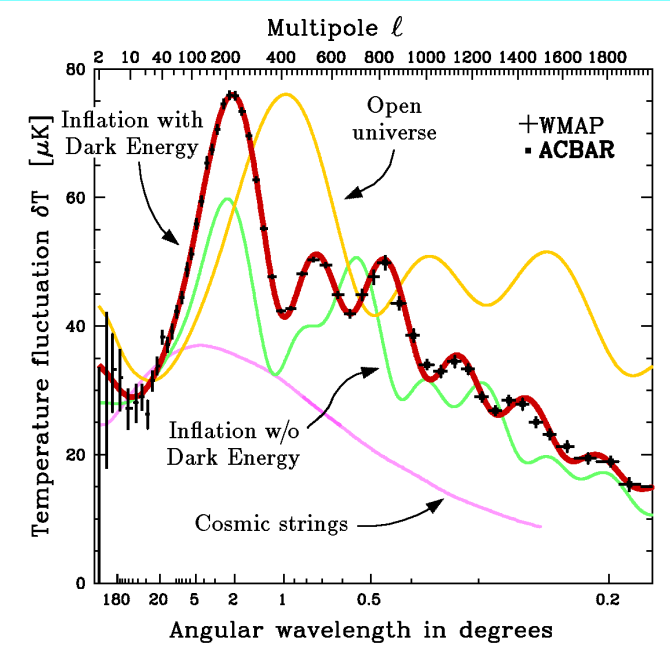
\includegraphics[width=250pt]{images/inflation predictions.png}
    \end{figure}

    In inflation you cannot predict the amplitude of these fluctuations, since that would require a deeper understanding of high energy physics, however you can compute the spectrum.
\end{enumerate}


\subsection*{Universe to Multiverse}

The repulsive gravity material that drives the inflation is metastable. In any one location, the probability of remaining in an inflating state decreases with time - usually exponentially. But, the Universe in the meantime is expanding exponentially. In any successful version of inflation, the exponential expansion is faster than the exponential decay! Therefore, the volume that is inflating increases with time, even though the inflating material is decaying! The inflation becomes eternal - once it starts, it never stops. The inflating region never disappears, but pieces of it undergo decay and produce "pocket universes," ad infinitum. Instead of one Universe, inflation produces an infinite number - \textbf{a multiverse}.


\subsection*{Dark Energy: Key Mystery of the Universe}

In 1998, astronomers discovered that the Universe has been accelerating for about the last 5 billion years (out of its 14 billion year history).

Implication: Inflation is happening today, so the Universe today is filled with a repulsive gravity material. (Within general relativity, this requires negative pressure.) The repulsive gravity material, which apparently fills space, is called the "DARK ENERGY". Nobody knows what dark energy is, but the simplest explanation is that its vacuum energy, also known as a cosmological constant.

The quantum vacuum is far from empty, so a nonzero energy density is no problem. In quantum field theory, the energy density of quantum fluctuations diverges. All wavelengths contribute, and there is no shortest wavelength. A plausible cutoff for the fluctuations is the Planck length, around $10^{-33}cm$, the scale of quantum gravity. Using thsi cutoff, the estimated vacuum energy density is too large. However it is too large by 120 orders of magnitude! lol


\subsection*{The Landscape of String Theory}

Since the inception of string theory, theorists have sought to find the vacuum of string theory - with no success. Within the past 20 years or so, most string theorists have come to the belief that there is no unique vacuum. Instead, there are maybe $10^{500}$ long-lived metastable states, any of which could serve as a substrate for a pocket Universe. This is the Landscape!

Eternal inflation can presumably produce an infinite number of pocket universes of every type, populating the landscape. Although string theory would govern everywhere, each type of vacuum would have its own low-energy physics - its own "standard model", its own "constants" of nature, and its own vacuum energy density.